\section{应用场景展望}
为了尊重资产的公平性,正当性,确权性,我们把分发模型的设计简洁、明了、有效。结合星云的生态特点,将更多的激励和博弈场景交给了应用场景本身,应用场景中的激励和消耗场景可以更加变化、多样。在本章节中,我们针对星云中已经存在的或是未来的应用场景进行一些展望,如图\ref{fig:nax_ecosys}所示,我们可以比较清晰的勾勒出NAX在星云生态的正向激励作用。

\begin{figure}[h]
  \centering
  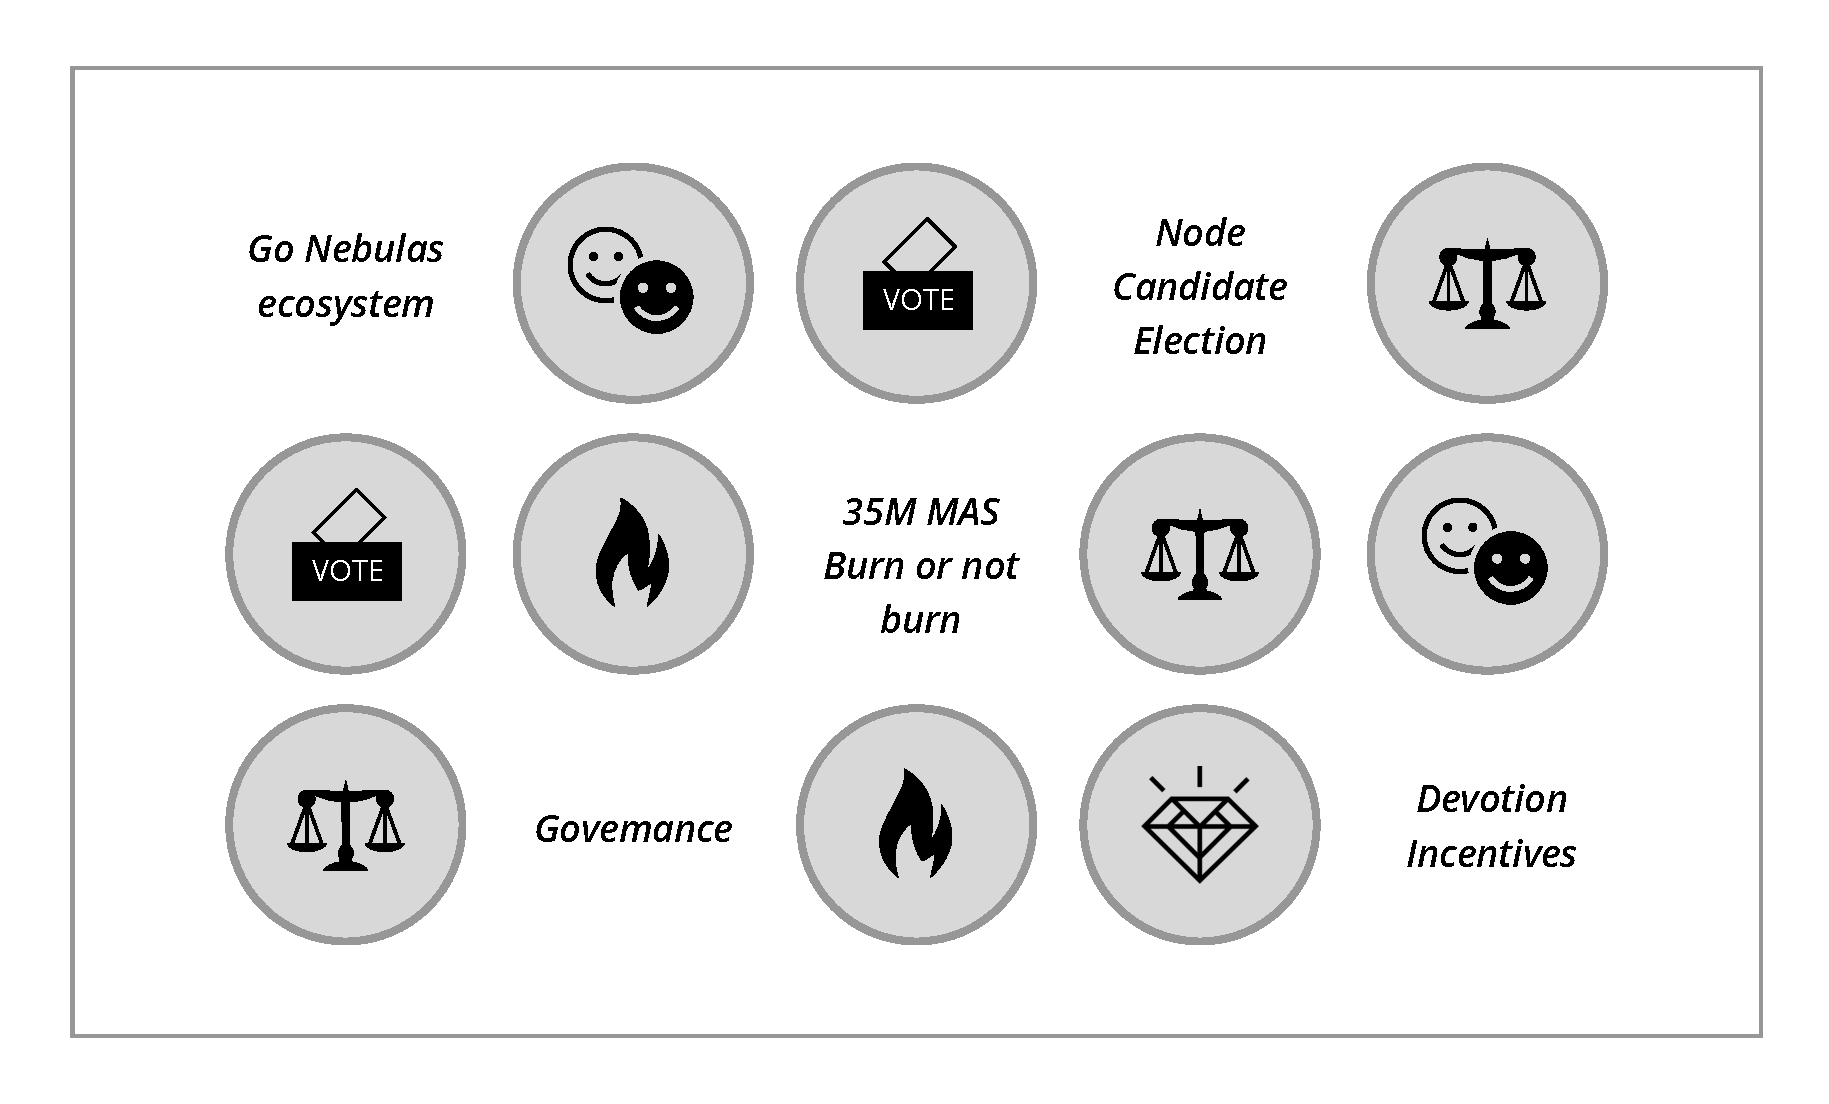
\includegraphics[width=0.6\textwidth]{../common/usecases.pdf}
  \caption{NAX在星云生态中的使用场景 \label{fig:nax_ecosys}}
\end{figure}

\subsection{生态贡献激励}
在白皮书中,从贡献证明的共识算法(PoD, Proof of Devotion),到星云的愿景的提出:在去中心化的协作中公平受益,再到2019年初,Go Nebulas平台的上线,都始终贯穿着星云对生态贡献度衡量的探索。这些都是星云进一步朝着Autonomous Metanet目标前进的重要环节。为此提出一种以质押投资基金为权益证明的激励方式,使之运用到不同场景的激励当中。具体的操作是,将项目投资基金(通常以NAS形式存在)进行质押,这部分资金质押所得的NAX权益,将作为该生态场景的NAX激励权益基金。

\subsubsection{Go Nebulas激励}
星云基金会将会投入不少于$3,000,000$NAS资金,用于资助Go Nebulas平台上的项目,而且根据需求,基金会还将随时追加资金的投入。这部分资金可以投入到质押当中,产生的权益将用来激励在Go Nebulas平台上做出不同贡献的权益证明,即在获得NAS资金作为报酬之外,还将获得由Go Nebulas平台制定的规则下的NAX激励,作为对星云生态做出贡献的权益,可以在星云生态上行使相应的权益和治理。详细的激励方案将由Go Nebulas的运营团队管理者或社区的参与者共同制定。激励可以分为以下几类:

\begin{enumerate}[\hspace{1cm}(a)]
  \item 核心基础建设
  \item 市场拓展
  \item 推广与邀新
  \item 提案与参与
\end{enumerate}

Go Nebulas平台除了是一个投入社区建设,获得NAX激励的重要方式之外,也同样是一个NAX的重要使用场景,消耗场景包含(不局限)于以下几类:
\begin{enumerate}[\hspace{1cm}(a)]
  \item 创建和发起提案
  \item 提案通过与否决
  \item 项目进行中的质押
\end{enumerate}

\subsubsection{基金会核心成员激励}
成为基金会核心团队的成员,包括兼职的人员,在获得相应的工资作为报酬之外,也将获得由基金会质押所产生的NAX权益作为额外的贡献证明。

\subsection{PoD共识探索}
随着星云对PoD研发的推进,去中心化是星云链的必由之路,NAX将可能在PoD中扮演重要角色,有效地结合主网正在研发的PoD技术创新成为新型共识算法的基础和方向。上一节讨论了NAX在生态中的激励场景, 加上NAX的单一的质押的发行方式,获得NAX的方式只能通过以下方式获得:
\begin{enumerate}[\hspace{1cm}(i)]
  \item 贡献资产的流动性
  \item 投入星云链建设
  \item 参与社区治理场景
\end{enumerate}

从另一外角度不难得出,NAX可以被看作为星云生态的贡献凭证。PoD顾名思义是贡献度证明,区别于PoW、PoS的本质在于,星云链更看中区块链协作当中,以不同角色对生态的贡献作为出块奖励的依据,而不仅依赖算力的大小或是筹码多寡。

在选择共识委员会的时候,可以引入NAX的权益多少来影响出块的概率大小。共识节点委员会的产生,无论是链下还是链上产生,NAX也将可以成为投票的重要依据。现在先链下节点竞选为例,阐述说明节点可能的方式,最终的形式将以官方发布的PoD技术文档为准:

\begin{enumerate}[\hspace{1cm}(a)]
  \item 节点委员会成员由NAX投票选出来
  \item 需要销毁相应量的NAX,并质押NAS
  \item 节点将分多个赛道,丰富生态多样性
  \item 主网PoD共识算法将引入NAX作为参数影响出块权益的分配
\end{enumerate}

\subsection{链上治理场景}
在星云生态的发展进程中,会出现各种各样的评选、选举等活动。为了提高社区生态中的参与度,每个活动将根据需要,使用NAX作为权益证明介质将会在投票和激励策略中发挥重要角色。

例如接下来关于如何处理社区预留的$35,000,000NAS$的方案,将成为比较早期的由社区来贡献方案,并由社区来投票决定处理方案的活动案例。星云基金会曾提议销毁,其中一种可能的方案是,每个月发起一次使用NAX的投票销毁社区预留剩余NAS总量的 \(\lambda\) \% , \(\lambda\) \% 是当前NAS质押率占流通总量的份额,我们也鼓励社区提供更加有效、积极的方案,共同决定这部分资产的使用。

\subsection{星云生态推广}
星云基金会扶持开发的,基础生态产品是星云链生态使用的重要入口,这里包含现在的,还有将来基金会孵化的星云生态产品,例如:NAS nano Pro~\cite{NASnano} 、Explorer~\cite{explorer}和Nebulas DEX等。随着NextDAO的推进以及社区治理的前进,社区里将会出现越来越多的NRC20 Token和治理尝试。这些币种有对生态工具的强烈需求,例如:NAS nano Pro和Explorer等。资源空间有限的情况下,为了使得星云生态相关的产品推出更多优秀好的项目,将可能会使用NAX作为平台征选优秀项目的工具以及保证金,这些保证金也同样可以作为生态项目的活动和激励经费,用于投入到平台的建设当中。
